%!TEX root = ../main.tex

En los capítulos \ref{chapter:BIN} y \ref{chapter:PO} trabajaremos con dos modelos de \lot para la representación de secuencias. Ambos trabajos se basan en variantes del \textit{lenguaje de geometría} presentado en~\cite{amalric2017language} para modelar el rendimiento humano de la memoria de trabajo en el dominio espacial de secuencias en un óctagono regular. Se ha demostrado previamente que este lenguaje predice para tres grupos poblacionales distintos (adultos educados, un pueblo del Amazonas sin educación formal y niños pequeños) qué secuencias aparecen como regulares y cómo se desempeñan en la tarea explícita de completar las secuencias mostradas~\cite{amalric2017language} o en la tarea implícita de seguimiento ocular de las secuencias~\cite{f60}. La complejidad de la secuencia, definida como una longitud mínima de descripción a partir de la gramática, también predijo la activación del cerebro humano en un amplio circuito cortical que incluía la corteza frontal inferior justo dorsal al área de Broca~\cite{f60}.

\section*{El lenguaje de geometría \gramgeo}

El \textit{lenguaje de geometría} permite la generación de programas que pueden codificar cualquier secuencia de ubicaciones espaciales en un octágono. Utiliza instrucciones primitivas (o producciones atómicas) que definen la magnitud y la dirección del siguiente paso (por ejemplo, \verb#+1# representa el siguiente elemento en el sentido de las agujas del reloj; \verb#+2#, el segundo elemento en el sentido de las agujas del reloj), así como la reflexión sobre algunos ejes (por ejemplo, \verb#H# representa la simetría horizontal, eligiendo la ubicación simétrica a lo largo de un eje horizontal). Además, estos elementos pueden concatenarse o repetirse, por ejemplo, \verb#REP0[+1]^8# describe un giro completo en el sentido de las agujas el reloj alrededor del octágono a partir de la repetición de la instrucción \verb#+1# ocho veces. Finalmente, estas instrucciones pueden anidarse arbitrariamente dando lugar a programas complejos a partir de la composición de subexpresiones.

\paragraph{La gramática \gramgeo.}
En la Figura \ref{fig:gramgeo} definimos la gramática para $\gramgeo$. Los {\em programas} de \gramgeo serán las palabras válidas del lenguaje definido por \gramgeo. Usaremos indistintamente \gramgeo para referirnos a la gramática o al lenguaje que representa (quedando siempre claro del contexto cuál de las dos aplica).

\renewcommand{\thefigure}{PI.1}
\begin{figure}
\begin{center}
\begin{tabular}{cc}

    \begin{minipage}[t]{0.35\textwidth}
    {\bf Símbolo inicial}

    \medskip

    \begin{tabular}{rcl}
    \start & $\to$ & \verb#[#\inst\verb#]# %& símbolo inicial 
    \end{tabular}

    \bigskip

    {\bf Producciones básicas}

    \medskip

    \begin{tabular}{rcl}
    \inst  & $\to$ & \atom %& producción atómica 
    \\
    \inst  & $\to$ & \inst\verb#,#\inst %& concatenación 
    \\
    \inst  & $\to$ & \rep\verb#[#\inst\verb#]^#$k$%& familia repetir con $n \in [2,8]$ 
    \\
    \rep  & $\to$ & \verb#REP0# %& repetición simple 
    \\

    \rep  & $\to$ & \verb#REP1<#\atom\verb#># %& repetir con variación del punto de inicio usando ATOMIC
    \\
    \rep  & $\to$ & \verb#REP2<#\atom\verb#># %& repetir con variación de la secuencia resultante usando ATOMIC
    \\
    \end{tabular}
    \end{minipage}
    
    \begin{minipage}[t]{0.35\textwidth}

    {\bf Producciones atómicas}

    \medskip

    \begin{tabular}{rcl}
    \atom  & $\to$ & \verb#-1# %& siguiente elemento en sentido antihorario (ACW) 
    \\
    \atom  & $\to$ & \verb#-2# %& segundo elemento ACW 
    \\
    \atom  & $\to$ & \verb#-3# %& tercer elemento ACW 
    \\
    \atom  & $\to$ & \verb#+0# %& permanecer en la misma posición 
    \\
    \atom  & $\to$ & \verb#+1# %& siguiente elemento en sentido horario (CW)
    \\
    \atom  & $\to$ & \verb#+2# %& segundo elemento CW 
    \\
    \atom  & $\to$ & \verb#+3# %& tercer elemento CW 
    \\
    \atom  & $\to$ & \verb#A # %& simetría alrededor de un eje diagonal 
    \\
    \atom  & $\to$ & \verb#B # %& simetría alrededor del otro eje diagonal 
    \\
    \atom  & $\to$ & \verb#H # %& simetría horizontal 
    \\
    \atom  & $\to$ & \verb#V # %& simetría vertical 
    \\
    \atom  & $\to$ & \verb#P # %& simetría rotacional 
    \end{tabular}
    \end{minipage}
\end{tabular}
\end{center}
\caption{La gramática \gramgeo donde $k$ es la representación en decimal de un número natural en el intervalo $\{2,\dots,8\}$}
\label{fig:gramgeo}
\end{figure}


\paragraph{La semántica de \gramgeo.}
Un programa $P$ por sí solo no tiene semántica, sino que la semántica viene dada por un par $(P,n)$, donde $P$ es un programa válido de \gramgeo y $n$ es un número natural entre 0 y 7. Denotaremos con $\sem{P}_n$ a la semántica de tal par, y será una secuencia no vacía de números naturales sobre el alfabeto $\{0,\dots,7\}$. Intuitivamente, $\sem{P}_n$ representa o describe un camino en el octágono de la Figura \ref{fig:circle}, cuando se `ejecuta' $P$ a partir del punto $n$. El mismo programa $P$ podrá describir distintas secuencias dependiendo del valor de $n$. 

\renewcommand{\thefigure}{PI.2}
\begin{figure}[ht]
\begin{center}
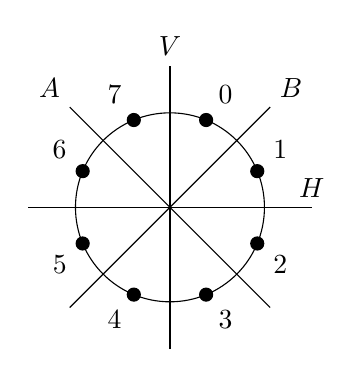
\begin{tikzpicture}[scale=.6]
\draw (-3,0) -- (3,0) node[above]{$H$};
\draw (0,-3) -- (0,3) node[above]{$V$};
\draw (-2.121320344,-2.121320344) -- (2.121320344,2.121320344) node[above right]{$B$};
\draw (2.121320344, -2.121320344) -- (-2.121320344,2.121320344) node[above left]{$A$};
\node at (0.765366865,  1.847759065) [circle,draw, scale=.5, fill, label=67.5:$0$]{};
\node at (1.847759065   , 0.765366865) [circle,draw, scale=.5, fill, label=22.5:$1$]{};
\node at (1.847759065   , -0.765366865) [circle,draw, scale=.5, fill, label=-22.5:$2$]{};
\node at (0.765366865   , -1.847759065) [circle,draw, scale=.5, fill, label=-67.5:$3$]{};
\node at (-0.765366865, -1.847759065) [circle,draw, scale=.5, fill, label=-112.5:$4$]{};
\node at (-1.847759065, -0.765366865) [circle,draw, scale=.5, fill, label=-157.5:$5$]{};
\node at (-1.847759065, 0.765366865) [circle,draw, scale=.5, fill, label=-202.5:$6$]{};
\node at (-0.765366865, 1.847759065) [circle,draw, scale=.5, fill, label=-247.5:$7$]{};
\draw (0,0) circle (2cm);
\end{tikzpicture}
\end{center}
   \caption{El octógono sobre el que \gramgeo describe caminos}\label{fig:circle}
\end{figure}

Se puede ver de la definición de la gramática \gramgeo que un programa $P$ será siempre de la forma 

\begin{center}
$P=$\verb#[# $I_1$ \verb#,# \dots \verb#,# $I_\ell$ \verb#]#
\end{center}

\noindent donde las $I_i$ serán {\em instrucciones} derivadas de \inst. La definición de la semántica formal la veremos más adelante.  Por ahora veamos informalmente la semántica de cada instrucción atómica, es decir, cualquier instrucción derivada del símbolo \atom\ en la gramática \gramgeo: 
\begin{itemize}
\item \verb#-1# representa siguiente elemento en sentido antihorario (SAH)

\item \verb#-2# representa el segundo elemento SAH

\item \verb#-3# representa el tercer elemento SAH 

\item \verb#+0# representa permanecer en la misma posición

\item \verb#+1# representa el siguiente elemento en sentido horario (SH)
 
\item \verb#+2# representa el segundo elemento SH

\item \verb#+3# representa el tercer elemento SH 

\item \verb#A# representa la simetría sobre un eje diagonal

\item \verb#B# representa la simetría sobre el otro eje diagonal 

\item \verb#H# representa la simetría horizontal 

\item \verb#V# representa la simetría vertical 

\item \verb#P# representa la simetría rotacional 
\end{itemize}

Además, \gramgeo tiene tres producciones que representan distintas formas de repeticiones de (sub)programas:

\begin{itemize}
\item Si $P$ es un programa, la ejecución de \verb#REP0[#$P$\verb#]^#$k$ desde $n$ será equivalente a la ejecución del siguiente programa: 

\begin{center}
%\verb#[# \underbrace{ $I_1$ \verb#,# \dots \verb#,# $I_\ell$ \verb#,#
%         $\dots$ \verb#,# 
%         $I_1$ \verb#,# \dots \verb#,# $I_\ell$}_\text{$k$ copias de $P$} \verb#]#
%\verb#[# $\underbrace{I_1, \dots, I_l, \dots, I_1, \dots, I_l}_\text{$k$ copias de $P$}$ \verb#]#

\begin{algorithm}
  \SetKwFunction{Print}{Print}
  \For{$i \gets 1$ \KwTo $k$}{
    $cadena \leftarrow \FuncSty{P(}n\FuncSty{)}$\;
    \Print{cadena}\;
    $n \leftarrow$ último símbolo de $cadena$
    }
\end{algorithm}


\end{center}



\item Si $A$ es una instrucción atómica y $P$ es un programa, la ejecución del programa 
\verb#REP1<#$A$\verb#>[#$P$\verb#]^#$k$ desde $n$ será equivalente a primero obtener la secuencia $\sigma_0$ resultante de ejecutar $P$ desde el punto $n$  y luego ejecutar $A$ desde cada punto de $\sigma_0$ para obtener $\sigma_1$, y repetir el procedimiento aplicando $A$ a cada punto de la última secuencia resultante hasta obtener $\sigma_{k-1}$. Es decir, con $\cdot\concat\cdot$ representando la concatenación de secuencias, entonces:

\begin{center}
\begin{algorithm}
  \SetKwFunction{Print}{Print}
  $cadena \leftarrow \FuncSty{P(}n\FuncSty{)}$\;
  \Print{cadena}\;
  \For{$i \gets 2$ \KwTo $k$}{
        $nueva \ cadena \leftarrow$ cadena vacía \;
        \ForEach{$simbolo \in cadena$}{
            $ res \leftarrow$ \FuncSty{A(}$simbolo$\FuncSty{)}\;
            $nueva \ cadena \leftarrow nueva \ cadena \concat res$\;
        }
        $cadena \leftarrow nueva \ cadena$\;
        \Print{cadena}
    }
\end{algorithm}
\end{center}


%$\llbracket$ \verb#REP1<#$A$\verb#>[#$P$\verb#]^#$k$  $\rrbracket_n = \sigma_0 \concat \dots \concat \sigma_{k-1}$

%donde
      
%      $\sigma_0 = \sem{P}_n = x_0^0 \concat \dots \concat x_i^0$
      
      %$\sigma_1 = \sem{A}_{x_0^0} \dots \sem{A}_{x_i^0} = x_0^1 \dots x_i^1$
      
      %$\sigma_2 = \sem{A}_{x_0^1} \dots \sem{A}_{x_i^1} = x_0^2 \dots x_i^2$
      
%      $\sigma_j = \sem{A}_{x_0^{j-1}} \concat \dots \concat \sem{A}_{x_i^{j-1}} = x_0^j \concat \dots \concat x_i^j$ para todo $j>0$



\item Si $A$ es una instrucción atómica y $P$ es un programa, la ejecución del programa 
\verb#REP2<#$A$\verb#>[#$P$\verb#]^#$k$ desde $n$ será equivalente a primero obtener la secuencia $\sigma_0$ resultante de ejecutar $P$ desde el punto $n$ y luego volver a ejecutar $P$ desde $\sem{A}_n$ para obtener $\sigma_1$, y repetir el procedimiento hasta obtener $\sigma_{k-1}$. Es decir,

\begin{center}
\begin{algorithm}
  \SetKwFunction{Print}{Print}
  \For{$i \gets 1$ \KwTo $k$}{
        $cadena \leftarrow$ \FuncSty{P(}$n$\FuncSty{)}\;
        \Print{cadena}\;
        $n \leftarrow \FuncSty{A(}n\FuncSty{)}$\;
    }
\end{algorithm}
\end{center}

%\begin{center}

%$\llbracket$ \verb#REP2<#$A$\verb#>[#$P$\verb#]^#$k$  $\rrbracket_n = \sigma_0 \concat \dots \concat \sigma_{k-1}$

%donde
      
%      $\sigma_i = \sem{P}_{n_i} $
      
%      con $n_0 = n$ y $n_i = \sem{A}_{n_{i-1}}$ para $i>0$ 


%\end{center}

\end{itemize}

Dado $\alpha$ un programa o una instrucción, y dado $n\in\{0,\dots,7\}$, definimos ahora formalmente $\sem{\alpha}_n$, la {\em semántica de $\alpha$ a partir de $n$}, recursivamente en la complejidad del árbol sintáctico de $\alpha$ en la gramática \gramgeo.

Definimos primero la semántica de las instrucciones atómicas de la siguiente forma:

\begin{tabular}{cc}
    \begin{minipage}[t]{0.45\textwidth}
        \begin{itemize}
        \item $\llbracket$\verb#+0#$\rrbracket_n  \eqdef  n$ 
        \item $\llbracket$\verb#+1#$\rrbracket_n  \eqdef  n+1 \mod 8$  
        \item $\llbracket$\verb#-1#$\rrbracket_n  \eqdef  n-1 \mod 8$  
        \item $\llbracket$\verb#+2#$\rrbracket_n  \eqdef  n+2 \mod 8$  
        \item $\llbracket$\verb#-2#$\rrbracket_n  \eqdef  n-2 \mod 8$  
        \item $\llbracket$\verb#+3#$\rrbracket_n  \eqdef  n+3 \mod 8$  
        \item $\llbracket$\verb#-3#$\rrbracket_n  \eqdef  n-3 \mod 8$  
        \end{itemize}
    \end{minipage}
    &
    \begin{minipage}[t]{0.45\textwidth}
        \begin{itemize}
        \item $\llbracket$\verb#P#$ \rrbracket_n  \eqdef  4+n \mod 8$  
        \item $\llbracket$\verb#H#$ \rrbracket_n  \eqdef  3-n \mod 8$  
        \item $\llbracket$\verb#V#$ \rrbracket_n  \eqdef  7-n \mod 8$  
        \item $\llbracket$\verb#A#$ \rrbracket_n  \eqdef  5-n \mod 8$  
        \item $\llbracket$\verb#B#$ \rrbracket_n  \eqdef  1-n \mod 8$  
        \end{itemize}
    \end{minipage}
\end{tabular}

\medskip

La semántica de las otras instrucciones (salvo la regla de que introduce `\verb#,#') es la siguiente:
\begin{itemize}
\item Si $I=$ \verb#REP0[#$P$\verb#]^#$k$, con $P$ un programa, 
definimos 
$\sem{I}_n \eqdef \sem{\underbrace{[P,\dots,P]}_\text{k veces}}_n $


\item Si $I=$ \verb#REP1<#$A$\verb#>[#$P$\verb#]^#$k$, con $P$ un programa y $A$ una instrucción atómica, 
definimos 
$\sem{I}_n \eqdef  \sigma_0 \concat \dots \concat \sigma_{k-1}$ donde
      
      $\sigma_0 = \sem{P}_n = x_0^0 \concat \dots \concat x_i^0$
      
      $\sigma_j = \sem{A}_{x_0^{j-1}} \concat \dots \concat \sem{A}_{x_i^{j-1}} = x_0^j \concat \dots \concat x_i^j$ para todo $j>0$ 
      
      $(x_i^j \in\{0,\dots,7\})$

\item Si $I=$ \verb#REP2<#$A$\verb#>[#$P$\verb#]^#$k$, con $P$ un programa y $A$ una instrucción atómica, 
definimos 
$\sem{I}_n \eqdef \underbrace{\sem{P}_{n_0} \concat \dots \concat \sem{P}_{n_i}}_\text{k veces}$ donde $n_0 = n$ y $n_i = \sem{A}_{n_{i-1}}$ para $i>0$ 
\end{itemize}

Finalmente, si $P=$ \verb#[# $I$ \verb#]#, entonces $\sem{P}_n\eqdef\sem{I}_n$, 
y si $P=$\verb#[# $I_1$ \verb#,# $I_2$ \verb#,# \dots \verb#,# $I_\ell$ \verb#]# con $\ell>1$, entonces

\begin{center}
$\sem{P}_n \eqdef \sem{I_1}_n \concat \llbracket$
\verb#[# $I_2$ \verb#,# \dots \verb#,# $I_\ell$ \verb#]#
$\rrbracket_m$
\end{center}

\noindent donde $m\in\{0,\dots,7\}$ es el último símbolo de la secuencia $\sem{I_1}_n$ 


\paragraph{Complejidad para \gramgeo.} 
Si $\alpha$ es un programa o una instrucción de \gramgeo, definimos el {\em tamaño} de $\alpha$, notado $|\alpha|$ de la siguiente manera:
%
\begin{itemize}
\item Si $\alpha$ es una instrucción atómica, $|\alpha|\eqdef 2$.

\item Si $\alpha$ es una instrucción de la forma 
\verb#REP0[#$P$\verb#]^#$k$, con $P$ un programa, 
entonces $|\alpha|\eqdef |P|+\lceil \log k\rceil$.

\item Si $\alpha$ es una instrucción de la forma 
\verb#REP1<#$A$\verb#>[#$P$\verb#]^#$k$ o de la forma 
\verb#REP2<#$A$\verb#>[#$P$\verb#]^#$k$ 
con $P$ un programa y $A$ una instrucción atómica, 
entonces $|\alpha|\eqdef |P|+\lceil \log k\rceil+|A|$.

\item Si $\alpha$ es un programa de la forma
\verb#[# $I_1$ \verb#,# $I_2$ \verb#,# \dots \verb#,# $I_\ell$ \verb#]#
entonces $|\alpha|\eqdef \sum_{i=1}^\ell|I_i|$.
\end{itemize}
%
Si $s$ es una secuencia no vacía sobre $\{0,\dots,7\}$, definimos la {\em $\gramgeo$-complejidad de la descripción mínima} de $s$, notada $\mdlgeo(s)$, como el tamaño del programa que, ejecutado desde 0, produce la secuencia $s$, es decir,
$$
\mdlgeo(s)\eqdef\min\{|P|\mid P\in\gramgeo,\sem{P}_0=s\}.
$$



\paragraph{Ejemplos}\santi{estos ejemplos no tendrían que estar antes del paragraph de complejidad?}

\begin{itemize}
\item  $\llbracket$\verb#[+1,-1]#$\rrbracket_1 = 21$

\item  $\llbracket$\verb#REP0[+0]^4#$\rrbracket_3 = 3333$

\item  $\llbracket$\verb#REP0[+1]^4#$\rrbracket_0 = 1234$

\item  $\llbracket$\verb#REP0[+1,-1]^3#$\rrbracket_1 = 212121$

\item  $\llbracket$\verb#[REP0[+1]^4, REP0[-2, REP0[+1]^3 ]^2]#$\rrbracket_0 = 123423453456$

\item  $\llbracket$\verb#REP1<+1>[REP0[+1]^4]^3#$\rrbracket_0 = 123423453456$

$= 1234 \ \ \concat \ \ \llbracket$\verb#+1#$\rrbracket_1 \concat \llbracket$\verb#+1#$\rrbracket_2 \concat \llbracket$\verb#+1#$\rrbracket_3 \concat \llbracket$\verb#+1#$\rrbracket_4 \ \ \concat \ \ \llbracket$\verb#+1#$\rrbracket_2 \concat \llbracket$\verb#+1#$\rrbracket_3 \concat \llbracket$\verb#+1#$\rrbracket_4 \concat \llbracket$\verb#+1#$\rrbracket_5$

\item  $\llbracket$\verb#REP2<-1>[REP0[V]^2]^4#$\rrbracket_3 = 43526170$ 

$= \llbracket$\verb#REP0[V]^2]#$ \rrbracket_3 \concat \llbracket$ \verb#REP0[V]^2]#$ \rrbracket_2 \concat \llbracket$ \verb#REP0[V]^2]#$ \rrbracket_1 \concat \llbracket$ \verb#REP0[V]^2]#$ \rrbracket_0$

\item  $\llbracket$ \verb#REP1<-1>[REP0[V]^2]^4#$\rrbracket_3 = 43322110$

$= 43 \ \ \concat \ \ \llbracket$\verb#-1#$\rrbracket_4 \concat \llbracket$\verb#-1#$\rrbracket_3 \ \ \concat \ \ \llbracket$\verb#-1#$\rrbracket_3 \concat \llbracket$\verb#-1#$\rrbracket_2 \ \ \concat \ \ \llbracket$\verb#-1#$\rrbracket_2 \concat \llbracket$\verb#-1#$\rrbracket_1 $

\end{itemize}


En el cuadro~\ref{PART1:Tabla:MDL} mostramos la complejidad \mdlgeo(s) para algunas secuencias $s$ junto con distintos programas $p \in$ \gramgeo tal que $\sem{p}_0=s$ y $|p|=\mdlgeo(s) $.


\renewcommand{\thetable}{PI.1}
\begin{table}[h!]
\centering
\begin{tabular}{lcl}
\multicolumn{1}{c}{ \boldmath{$s$}   } & \multicolumn{1}{c}{$\mdlgeo(s)$} & \multicolumn{1}{c}{Posibles $p$}  \\ \hline
\textbf{01234567} &  7      &  \begin{minipage}[t]{5cm}\verb#[+0,REP0[+1]^7]# \\  \verb#[REP1<+1>[+0]^8]#\end{minipage} \\ \hline
\textbf{02460246} &  7      &  \begin{minipage}[t]{5cm}\verb#[+0,REP0[+2]^7]# \\  \verb#[REP2<+2>[+0]^8]#\end{minipage} \\ \hline
\textbf{04512673} &  8      &  \begin{minipage}[t]{5cm}\verb#[REP1<-3>[+0,P]^4]# \\  \verb#[REP2<-3>[+0,P]^4]#\end{minipage} \\ \hline
\textbf{0213243546576071} &  9 &  \begin{minipage}[t]{5cm}\verb#[REP1<+1>[+0,+2]^8]# \\  \verb#[REP2<+1>[+0,+2]^8]#\end{minipage} \\ \hline
\textbf{02360236} &  11      &  \begin{minipage}[t]{5cm}\verb#[REP1<+0>[+0,+2,A,B]^2]# \\  \verb#[REP1<+0>[+0,+2,+1,+3]^2]#\end{minipage} \\ \hline
\end{tabular}
\caption{Secuencias $s$ y posibles $p$ con $\sem{p}_0=s$ y $|p|=\mdlgeo(s)$} \label{PART1:Tabla:MDL}
\end{table}




\color{black}

\section*{El lenguaje de geometría en secuencias binarias: \grambin}

En el capítulo \ref{chapter:PO}, probamos la hipótesis de que el lenguaje \gramgeo, cuando se reduce a sólo dos ubicaciones, es suficiente para dar cuenta de la codificación humana en un tipo completamente diferente de secuencias: un dominio no espacial (auditivo y visual) de secuencias binarias compuestas por sólo dos estados arbitrarios A y B en lugar de las ocho ubicaciones del octágono. 

Para tales secuencias, el lenguaje puede ser despojado de la mayoría de sus instrucciones atómicas. Sólo mantuvimos las operaciones de permanecer en la misma posición (\verb#+0#), y de pasar al otro elemento (aquí denotado \verb#B#, es decir, la instrucción de alternancia, pero equivalente a la simetría de puntos \verb#P# en el lenguaje original). Por otro lado, se mantuvieron las tres variantes de repeticiones: \verb#REP0#, \verb#REP1# y \verb#REP2#, así como la capacidad de anidamiento de expresiones. 

\paragraph{La gramática \grambin.}
En la Figura \ref{fig:grambin} definimos la gramática para $\grambin$. Los {\em programas} de \grambin serán las palabras válidas del lenguaje definido por \grambin. Al igual que para el lenguaje anterior, usaremos indistintamente \grambin para referirnos a la gramática o al propio lenguaje que representa (quedando siempre claro del contexto cuál de las dos aplica).

\renewcommand{\thefigure}{PI.3}
\begin{figure}
\begin{center}
\begin{tabular}{cc}

    \begin{minipage}[t]{0.35\textwidth}
    {\bf Símbolo inicial}

    \medskip

    \begin{tabular}{rcl}
    \start & $\to$ & \verb#[#\inst\verb#]# %& símbolo inicial 
    \end{tabular}

    \bigskip

    {\bf Producciones básicas}

    \medskip

    \begin{tabular}{rcl}
    \inst  & $\to$ & \atom %& producción atómica 
    \\
    \inst  & $\to$ & \inst\verb#,#\inst %& concatenación 
    \\
    \inst  & $\to$ & \rep\verb#[#\inst\verb#]^#$k$%& familia repetir con $n \in [2,8]$ 
    \\
    \rep  & $\to$ & \verb#REP0# %& repetición simple 
    \\

    \rep  & $\to$ & \verb#REP1<#\atom\verb#># %& repetir con variación del punto de inicio usando ATOMIC
    \\
    \rep  & $\to$ & \verb#REP2<#\atom\verb#># %& repetir con variación de la secuencia resultante usando ATOMIC
    \\
    \end{tabular}
    \end{minipage}
    
    \begin{minipage}[t]{0.35\textwidth}

    {\bf Producciones atómicas}

    \medskip

    \begin{tabular}{rcl}    \\
    \atom  & $\to$ & \verb#+0# %& permanecer en la misma posición 
    \\
    \atom  & $\to$ & \verb#B # %& simetría alrededor del otro eje diagonal 
    \end{tabular}
    \end{minipage}
\end{tabular}
\end{center}
\caption{La gramática \grambin donde $k$ es la representación en decimal de un número natural}
\label{fig:grambin}
\end{figure}

\paragraph{La semántica de \grambin.}

Al igual que en \grambin, la semántica de un programa $P$ viene dada por un par $(P,n)$, donde $P$ es un programa válido de \grambin y $n$ es un número natural entre 0 y 1 en este caso. Denotaremos con $\sem{P}_n$ a la semántica de tal par, y será una secuencia no vacía de números naturales sobre el alfabeto $\{0,1\}$. Intuitivamente, $\sem{P}_n$ representa o describe una secuencia binaria, cuando se `ejecuta' $P$ a partir del símbolo $0$ o del símbolo $1$. 

Si bien aquí utilizaremos los símbolos $0$ y $1$ en la definición de la semántica para mostrar su relación con el lenguaje anterior, en el capítulo~\ref{chapter:BIN} nos referiremos a los símbolos $A$ y $B$ de las secuencias binarias para facilitar la lectura.

La definición de la gramática \grambin respeta las mismas reglas que \gramgeo. Simplemente, se reducen las instrucción atómicas a sólo dos opciones: 
\begin{itemize}

\item \verb#+0# representa permanecer en el símbolo actual

\item \verb#B# representa alternar el símbolo actual 

\end{itemize}

Formalmente,\santi{podemos simplemente poner $1-n$? y aclarar que $n$ es 0 o 1}

\begin{tabular}{cc}
    \begin{minipage}[t]{0.45\textwidth}
        \begin{itemize}
        \item $\llbracket$\verb#+0#$\rrbracket_n  \eqdef  n$ 
        \item $\llbracket$\verb#B#$ \rrbracket_n  \eqdef  1-n \mod 2$  
        \end{itemize}
    \end{minipage}
\end{tabular}

\medskip

La semántica de las producciones básicas se mantiene igual que en \gramgeo.

\paragraph{Complejidad para \grambin.} 

Si $\alpha$ es un programa o una instrucción de \grambin, definimos el {\em tamaño} de $\alpha$, notado $|\alpha|$ exactamente igual que para \grambin. Es decir:
%
\begin{itemize}
\item Si $\alpha$ es una instrucción atómica, $|\alpha|\eqdef 2$.

\item Si $\alpha$ es una instrucción de la forma 
\verb#REP0[#$P$\verb#]^#$k$, con $P$ un programa, 
entonces $|\alpha|\eqdef |P|+\lceil \log k\rceil$.

\item Si $\alpha$ es una instrucción de la forma 
\verb#REP1<#$A$\verb#>[#$P$\verb#]^#$k$ o de la forma 
\verb#REP2<#$A$\verb#>[#$P$\verb#]^#$k$ 
con $P$ un programa y $A$ una instrucción atómica, 
entonces $|\alpha|\eqdef |P|+\lceil \log k\rceil+|A|$.

\item Si $\alpha$ es un programa de la forma
\verb#[# $I_1$ \verb#,# $I_2$ \verb#,# \dots \verb#,# $I_\ell$ \verb#]#
entonces $|\alpha|\eqdef \sum_{i=1}^\ell|I_i|$.
\end{itemize}
%
Si $s$ es una secuencia no vacía sobre $\{0,1\}$, definimos la {\em $\grambin$-complejidad de la descripción mínima} de $s$, notada $\mdlbin(s)$, como el tamaño del programa que, ejecutado desde 0, produce la secuencia $s$, es decir,
$$
\mdlbin(s)\eqdef\min\{|P|\mid P\in\grambin,\sem{P}_0=s\}.
$$


El código de ambos lenguajes y del cálculo de las complejidades se encuentra disponible en \hyperref[https://github.com/sromano/language-of-geometry]{\url{https://github.com/sromano/language-of-geometry}}

\renewcommand{\thetable}{\arabic{chapter}.\arabic{figure}}
\renewcommand{\thefigure}{\arabic{chapter}.\arabic{figure}}